% answers.tex —— 2006 年·普通高等学校招生考试·山东卷理科 · 参考答案与详细解析片段
% 由 tools/generate_projects.py 依来源总账自 2006/2006_数学真题_山东理_试题.md + 2006/2006_数学真题_山东理_解析正文.md + 2006/2006_数学真题_山东理_答案要点.md 生成，勿手改（改源 MD 后重跑）


\begin{gktip}
以下推导仅依据固定候选题面，由本库独立求解，不是官方解析。固定 PDF 未见答案或解析页；Q5、Q10 按固定题面推导与选项不一致，暂记 U/PENDING，不补猜。
\end{gktip}

\begin{answer}
\gksolhead{1}{}

\textbf{题目}：

\Needspace{5\baselineskip}
定义集合运算
\nopagebreak[4]
\[
A\odot B=\{z\mid z=xy(x+y),\ x\in A,\ y\in B\}.
\]
设集合 $A=\{0,1\}$，$B=\{2,3\}$，则集合 $A\odot B$ 的所有元素之和为\mbox{（　　）}。

（A）$0$　　（B）$6$　　（C）$12$　　（D）$18$

\Needspace{4\baselineskip}
\textbf{解析}

取 $x=0$ 得到 $0$；取 $x=1$、$y=2,3$ 分别得到 $6,12$。集合 $A\odot B=\{0,6,12\}$，元素和为 $18$，选 D。

\gkanswer{答案：D（18）。}

\end{answer}
\begin{answer}
\gksolhead{2}{}

\textbf{题目}：

函数 $y=1+a^x\ (0<a<1)$ 的反函数的图象大致是\mbox{（　　）}。
\nopagebreak[4]
\begin{center}% 来源：固定候选 PDF，山东理科，PDF 第1页（印刷页320），Q2 四选项。
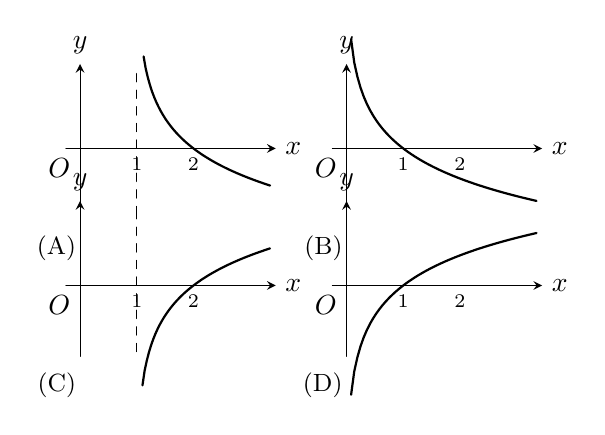
\begin{tikzpicture}[x=0.72cm,y=0.58cm,>=stealth,line cap=round,line join=round]
\tikzset{axis/.style={->,thin},curve/.style={thick},asym/.style={dashed,thin}}
\foreach \x/\y/\idx/\lbl in {0/3/0/A,4.7/3/1/B,0/0/2/C,4.7/0/3/D}{
  \begin{scope}[shift={(\x,\y)}]
    \draw[axis] (-0.25,0)--(3.45,0) node[right] {$x$};
    \draw[axis] (0,-1.55)--(0,1.85) node[above] {$y$};
    \node[below left] at (0,0) {$O$};
    \node[below] at (1,0) {\scriptsize 1};
    \node[below] at (2,0) {\scriptsize 2};
    \node[below left] at (0.1,-1.7) {\small (\lbl)};
    \ifcase\idx
      \draw[asym] (1,-1.45)--(1,1.7);
      \draw[curve,domain=1.12:3.35,samples=60] plot (\x,{ -0.95*ln(\x-1) });
    \or
      \draw[curve,domain=0.08:3.35,samples=60] plot (\x,{ -0.95*ln(\x) });
    \or
      \draw[asym] (1,-1.45)--(1,1.7);
      \draw[curve,domain=1.1:3.35,samples=60] plot (\x,{ 0.95*ln(\x-1) });
    \or
      \draw[curve,domain=0.08:3.35,samples=60] plot (\x,{ 0.95*ln(\x) });
    \fi
  \end{scope}
}
\end{tikzpicture}
\end{center}
\nopagebreak[4]
\Needspace{4\baselineskip}
\textbf{解析}

由 $y=1+a^x$ 解得反函数 $y=\log_a(x-1)$，定义域为 $x>1$，在 $x=1$ 有垂直渐近线，且递减并经过 $(2,0)$，对应选项 A。

\gkanswer{答案：A。}

\end{answer}
\begin{answer}
\gksolhead{3}{}

\textbf{题目}：

\Needspace{5\baselineskip}
设
\nopagebreak[4]
\[
f(x)=\begin{cases}
2e^{x-1}, & x<2,\\
\log_3(x^2-1), & x\ge 2,
\end{cases}
\]
则不等式 $f(x)>2$ 的解集为\mbox{（　　）}。

（A）$(1,2)\cup(3,+\infty)$　　（B）$(\sqrt{10},+\infty)$

（C）$(1,2)\cup(\sqrt{10},+\infty)$　　（D）$(1,2)$

\Needspace{4\baselineskip}
\textbf{解析}

当 $x<2$ 时，$2e^{x-1}>2$ 等价于 $x>1$，得到 $(1,2)$。当 $x\ge2$ 时，$\log_3(x^2-1)>2$ 等价于 $x^2>10$，得到 $(\sqrt{10},+\infty)$。合并得 $(1,2)\cup(\sqrt{10},+\infty)$，选 C。

\gkanswer{答案：C。}

\end{answer}
\begin{answer}
\gksolhead{4}{}

\textbf{题目}：

在 $\triangle ABC$ 中，角 $A,B,C$ 的对边分别为 $a,b,c$。已知 $A=\dfrac{\pi}{3}$，$a=\sqrt3$，$b=1$，则 $c=$\mbox{（　　）}。

（A）$1$　　（B）$2$　　（C）$\sqrt3-1$　　（D）$\sqrt3$

\Needspace{4\baselineskip}
\textbf{解析}

余弦定理给出 $a^2=b^2+c^2-2bc\cos A$，即 $3=1+c^2-c$。正根为 $c=2$，选 B。

\gkanswer{答案：B（2）。}

\end{answer}
\begin{answer}
\gksolhead{5}{}

\textbf{题目}：

设向量 $\vec a=(1,-2)$，$\vec b=(-2,4)$，$\vec c=(-1,-2)$。若表示向量 $4\vec a$、$4\vec b-2\vec c$、$2(\vec a-\vec c)$、$\vec d$ 的有向线段首尾相接能构成四边形，则向量 $\vec d$ 为\mbox{（　　）}。

（A）$(2,6)$　　（B）$(-2,6)$　　（C）$(2,-6)$　　（D）$(-2,-6)$

\Needspace{4\baselineskip}
\textbf{解析}

\Needspace{5\baselineskip}
四个向量首尾相接闭合要求其和为零。前三个向量之和为
\nopagebreak[4]
\[
4\vec a+(4\vec b-2\vec c)+2(\vec a-\vec c)
=6\vec a+4\vec b-4\vec c
=(2,12).
\]
所以 $\vec d=(-2,-12)$，但该向量不在题面选项中。固定副本未提供可裁决的勘误或另一个答案来源，故保留 U/PENDING，不选取近似选项。

\gkanswer{答案：U/PENDING；闭合向量为 $(-2,-12)$，不在选项中，见解析。}

\end{answer}
\begin{answer}
\gksolhead{6}{}

\textbf{题目}：

已知定义在 $\mathbb R$ 上的奇函数 $f(x)$ 满足 $f(x+2)=-f(x)$，则 $f(6)$ 的值为\mbox{（　　）}。

（A）$-1$　　（B）$0$　　（C）$1$　　（D）$2$

\Needspace{4\baselineskip}
\textbf{解析}

奇函数给出 $f(0)=0$。由 $f(x+2)=-f(x)$ 递推，$f(2)=f(4)=f(6)=0$，选 B。

\gkanswer{答案：B（0）。}

\end{answer}
\begin{answer}
\gksolhead{7}{}

\textbf{题目}：

在给定椭圆中，过焦点且垂直于长轴的弦长为 $\sqrt2$，焦点到相应准线的距离为 $1$，则该椭圆的离心率为\mbox{（　　）}。

（A）$\sqrt2$　　（B）$\dfrac{\sqrt2}{2}$　　（C）$\dfrac12$　　（D）$\dfrac{\sqrt2}{4}$

\Needspace{4\baselineskip}
\textbf{解析}

设椭圆半长轴为 $a$、焦距参数为 $c$、离心率 $e=c/a$。焦点处垂直于长轴的弦长为通径 $2b^2/a=2a(1-e^2)=\sqrt2$；焦点到同侧准线的距离为 $a/e-c=a(1-e^2)/e=1$。两式相除得到 $2e=\sqrt2$，故 $e=\sqrt2/2$，选 B。

\gkanswer{答案：B（$\sqrt2/2$）。}

\end{answer}
\begin{answer}
\gksolhead{8}{}

\textbf{题目}：

设 $p\colon x^2-x-20>0$，$q\colon\dfrac{1-x^2}{|x|-2}<0$，则 $p$ 是 $q$ 的\mbox{（　　）}。

（A）充分不必要条件　　（B）必要不充分条件

（C）充要条件　　（D）既不充分也不必要条件

\Needspace{4\baselineskip}
\textbf{解析}

令 $t=|x|$。$q$ 中分子 $1-t^2$ 在 $t=1$ 处变号，分母 $t-2$ 在 $t=2$ 处变号，故 $q$ 的解为 $|x|<1$ 或 $|x|>2$。而 $p$ 的解为 $x<-4$ 或 $x>5$，所以 $p\Rightarrow q$，反向不成立，选 A。

\gkanswer{答案：A（充分不必要条件）。}

\end{answer}
\begin{answer}
\gksolhead{9}{}

\textbf{题目}：

已知集合 $A=\{5\}$，$B=\{1,2\}$，$C=\{1,3,4\}$。从这三个集合各取一个元素构成空间直角坐标系中点的坐标，则确定的不同点的个数为\mbox{（　　）}。

（A）$33$　　（B）$34$　　（C）$35$　　（D）$36$

\Needspace{4\baselineskip}
\textbf{解析}

把取出的三个数放入有序坐标，先选 $5$ 的坐标轴，有 $3$ 种。其余两个坐标轴分别从 $B,C$ 或 $C,B$ 取数，$B\times C$ 与 $C\times B$ 各有 $6$ 种，交集仅为重复数对 $(1,1)$，故每个 $5$ 的位置有 $6+6-1=11$ 种，总数 $3\cdot11=33$，选 A。

\gkanswer{答案：A（33）。}

\end{answer}
\begin{answer}
\gksolhead{10}{}

\textbf{题目}：

已知 $\left(x^3-\dfrac{i}{\sqrt{x}}\right)^n$ 的展开式中第三项与第五项的系数之比为 $-\dfrac3{14}$，其中 $i^2=-1$，则展开式中的常数项是\mbox{（　　）}。

（A）$-45i$　　（B）$45i$　　（C）$-45$　　（D）$45$

\Needspace{4\baselineskip}
\textbf{解析}

\Needspace{5\baselineskip}
通项为
\nopagebreak[4]
\[
\binom nk x^{3n-7k/2}(-i)^k.
\]
\Needspace{5\baselineskip}
第三项与第五项的系数分别为 $-\binom n2$ 与 $\binom n4$。由其比值
\nopagebreak[4]
\[
-\frac{\binom n2}{\binom n4}=-\frac3{14}
\]
得 $(n-2)(n-3)=56$，正整数解为 $n=10$。常数项还需 $30-7k/2=0$，即 $k=60/7$，不是整数，不存在常数项；这与题面所给四个选项不符。保留 U/PENDING。

\gkanswer{答案：U/PENDING；按题面指数没有常数项，见解析。}

\end{answer}
\begin{answer}
\gksolhead{11}{}

\textbf{题目}：

\Needspace{5\baselineskip}
某公司招收男职员 $x$ 名、女职员 $y$ 名，$x$ 和 $y$ 须满足约束条件
\nopagebreak[4]
\[
\begin{cases}
5x-11y\ge -22,\\
2x+3y\ge 9,\\
2x\le 11,
\end{cases}
\]
则 $z=10x+10y$ 的最大值是\mbox{（　　）}。

（A）$80$　　（B）$85$　　（C）$90$　　（D）$95$

\Needspace{4\baselineskip}
\textbf{解析}

$x,y$ 为人数的非负整数。由 $2x\le11$ 得 $x\le5$，由 $5x-11y\ge-22$ 得 $y\le(5x+22)/11$。当 $x=5$ 时，$y\le4$，且 $(x,y)=(5,4)$ 满足 $2x+3y\ge9$，目标值 $10(x+y)=90$。对 $x\le4$，整数上界给出 $y\le3$，故目标值至多 $70$，最大值为 $90$，选 C。

\gkanswer{答案：C（90）。}

\end{answer}
\begin{answer}
\gksolhead{12}{}

\textbf{题目}：

如图，在等腰梯形 $ABCD$ 中，$AB=2DC=2$，$\angle DAB=60^\circ$，$E$ 为 $AB$ 的中点。将 $\triangle ADE$ 与 $\triangle BEC$ 分别沿 $ED$、$EC$ 向上折起，使 $A,B$ 重合于点 $P$，则三棱锥 $P-DCE$ 的外接球的体积为\mbox{（　　）}。

（A）$\dfrac{4\sqrt3\pi}{27}$　　（B）$\dfrac{\sqrt6\pi}{2}$

（C）$\dfrac{\sqrt6\pi}{8}$　　（D）$\dfrac{\sqrt6\pi}{24}$
\nopagebreak[4]
\begin{center}% 来源：固定候选 PDF，山东理科，PDF 第1页（印刷页320），Q12。
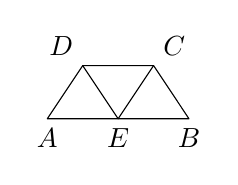
\begin{tikzpicture}[x=0.9cm,y=0.78cm,line cap=round,line join=round]
\coordinate (A) at (0,0); \coordinate (E) at (1,0); \coordinate (B) at (2,0);
\coordinate (D) at (0.5,0.866); \coordinate (C) at (1.5,0.866);
\draw (A)--(D)--(C)--(B)--cycle;
\draw (D)--(E)--(C);
\node[below] at (A) {$A$}; \node[below] at (E) {$E$}; \node[below] at (B) {$B$};
\node[above left] at (D) {$D$}; \node[above right] at (C) {$C$};
\end{tikzpicture}
\end{center}
\nopagebreak[4]
\Needspace{4\baselineskip}
\textbf{解析}

取 $AB=2$、$DC=1$，且 $E$ 为 $AB$ 中点。等腰梯形的腰长为 $1$，结合 $\angle DAB=60^\circ$ 可得 $AD=AE=DE=1$；同理 $BE=CE=BC=1$。折叠后 $A,B$ 重合于 $P$，各面边长保持不变，四面体 $P-DCE$ 的六条棱都为 $1$，是正四面体。其外接球半径 $R=\sqrt6/4$，体积为 $4\pi R^3/3=\sqrt6\pi/8$，选 C。

\gkanswer{答案：C（$\sqrt6\pi/8$）。}

\end{answer}
\begin{answer}
\gksolhead{13}{}

\textbf{题目}：

\Needspace{5\baselineskip}
若
\nopagebreak[4]
\[
\lim_{n\to\infty}\frac{1}{\sqrt n\left(\sqrt{n+a}-\sqrt n\right)}=1,
\]
则常数 $a=$\gkblank{}。

\Needspace{4\baselineskip}
\textbf{解析}

\Needspace{5\baselineskip}
有理化得
\nopagebreak[4]
\[
\frac{1}{\sqrt n(\sqrt{n+a}-\sqrt n)}
=\frac{\sqrt{n+a}+\sqrt n}{a\sqrt n}
\longrightarrow\frac2a.
\]
极限为 $1$，所以 $a=2$。

\gkanswer{答案：2。}

\end{answer}
\begin{answer}
\gksolhead{14}{}

\textbf{题目}：

已知抛物线 $y^2=4x$，过点 $P(4,0)$ 的直线与抛物线相交于 $A(x_1,y_1)$、$B(x_2,y_2)$ 两点，则 $y_1^2+y_2^2$ 的最小值是\gkblank{}。

\Needspace{4\baselineskip}
\textbf{解析}

\Needspace{5\baselineskip}
非竖直直线设为 $y=m(x-4)$，其中 $m\ne0$。代入 $y^2=4x$，交点横坐标和为 $x_1+x_2=8+4/m^2$。因 $y_i^2=4x_i$，有
\nopagebreak[4]
\[
y_1^2+y_2^2=4(x_1+x_2)=32+\frac{16}{m^2}>32.
\]
竖直线 $x=4$ 与抛物线交于 $y=\pm4$，取到 $32$，故最小值为 $32$。

\gkanswer{答案：32。}

\end{answer}
\begin{answer}
\gksolhead{15}{}

\textbf{题目}：

如图，已知在正三棱柱 $ABC-A_1B_1C_1$ 中所有棱长都相等，$D$ 是 $A_1C_1$ 的中点，则直线 $AD$ 与平面 $B_1DC$ 所成角的正弦值为\gkblank{}。
\nopagebreak[4]
\begin{center}% 来源：固定候选 PDF，山东理科，PDF 第1页（印刷页320），Q15。
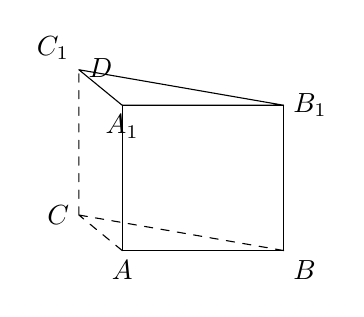
\begin{tikzpicture}[x=1cm,y=0.82cm,>=stealth,line cap=round,line join=round]
\coordinate (A) at (0,0); \coordinate (B) at (2.05,0);
\coordinate (C) at (-0.55,0.55); \coordinate (A1) at (0,2.25);
\coordinate (B1) at (2.05,2.25); \coordinate (C1) at (-0.55,2.80);
\coordinate (D) at (-0.275,2.525);
\draw (A)--(B) (A)--(A1) (B)--(B1);
\draw (A1)--(B1)--(C1)--cycle;
\draw[dashed] (A)--(C) (B)--(C) (C)--(C1);
\node[below] at (A) {$A$}; \node[below right] at (B) {$B$};
\node[left] at (C) {$C$}; \node[below] at (A1) {$A_1$};
\node[right] at (B1) {$B_1$}; \node[above left] at (C1) {$C_1$};
\node[above] at (D) {$D$};
\end{tikzpicture}
\end{center}
\nopagebreak[4]
\Needspace{4\baselineskip}
\textbf{解析}

\Needspace{5\baselineskip}
令棱长为 $1$，取
\nopagebreak[4]
\[
A=(0,0,0),\ B=(1,0,0),\ C=(1/2,\sqrt3/2,0),\ A_1=(0,0,1),\ B_1=(1,0,1),\ C_1=(1/2,\sqrt3/2,1),
\]
\Needspace{5\baselineskip}
则 $D=(A_1+C_1)/2=(1/4,\sqrt3/4,1)$。平面 $B_1DC$ 的法向量可取
\nopagebreak[4]
\[
\vec n=(-\sqrt3/4,-3/4,-\sqrt3/4),
\]
\Needspace{5\baselineskip}
而 $\overrightarrow{AD}=(1/4,\sqrt3/4,1)$。直线与平面的夹角 $\theta$ 满足
\nopagebreak[4]
\[
\sin\theta=\frac{|\overrightarrow{AD}\cdot\vec n|}{|AD|\,|\vec n|}
=\frac45.
\]

\gkanswer{答案：$4/5$。}

\end{answer}
\begin{answer}
\gksolhead{16}{}

\textbf{题目}：

下列四个命题中，真命题的序号有\gkblank{}。（写出所有真命题的序号）

① 将函数 $y=|x+1|$ 的图象按向量 $\vec v=(-1,0)$ 平移，得到的图象对应的函数表达式为 $y=|x|$；

② 圆 $x^2+y^2+4x+2y+1=0$ 与直线 $y=\dfrac12x$ 相交，所得弦长为 $2$；

③ 若 $\sin(\alpha+\beta)=\dfrac12$，$\sin(\alpha-\beta)=\dfrac13$，则 $\tan\alpha\cot\beta=5$；

④ 如图，已知正方体 $ABCD-A_1B_1C_1D_1$，$P$ 为底面 $ABCD$ 内一动点，$P$ 到平面 $AA_1D_1D$ 的距离与到直线 $CC_1$ 的距离相等，则 $P$ 点的轨迹是抛物线的一部分。
\nopagebreak[4]
\begin{center}% 来源：固定候选 PDF，山东理科，PDF 第1页（印刷页320），Q16。
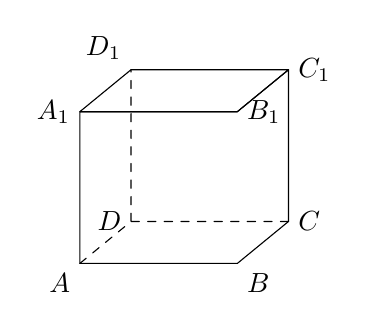
\begin{tikzpicture}[x=1cm,y=0.82cm,line cap=round,line join=round]
\coordinate (A) at (0,0); \coordinate (B) at (2,0); \coordinate (C) at (2.65,0.65); \coordinate (D) at (0.65,0.65);
\coordinate (A1) at (0,2.35); \coordinate (B1) at (2,2.35); \coordinate (C1) at (2.65,3); \coordinate (D1) at (0.65,3);
\draw (A)--(B)--(C)--(C1)--(B1)--(A1)--cycle;
\draw (A1)--(B1) (B1)--(C1) (D1)--(C1) (A1)--(D1);
\draw[dashed] (A)--(D) (D)--(C) (D)--(D1);
\node[below left] at (A) {$A$}; \node[below right] at (B) {$B$};
\node[right] at (C) {$C$}; \node[left] at (D) {$D$};
\node[left] at (A1) {$A_1$}; \node[right] at (B1) {$B_1$};
\node[right] at (C1) {$C_1$}; \node[above left] at (D1) {$D_1$};
\end{tikzpicture}
\end{center}
\nopagebreak[4]
\Needspace{4\baselineskip}
\textbf{解析}

① 图象左移 $1$ 个单位后对应 $y=|x+2|$，不是 $y=|x|$，错误。② 圆化为 $(x+2)^2+(y+1)^2=4$，圆心 $(-2,-1)$ 在直线 $y=x/2$ 上，弦长为直径 $4$，不是 $2$，错误。③ 将两式相加、相减得 $2\sin\alpha\cos\beta=5/6$、$2\cos\alpha\sin\beta=1/6$，故 $\tan\alpha\cot\beta=5$，正确。④ 点 $P$ 到平面 $AA_1D_1D$ 的距离等于其在底面内到直线 $AD$ 的距离；到直线 $CC_1$ 的距离等于到底面点 $C$ 的距离。等距轨迹是以 $C$ 为焦点、$AD$ 为准线的抛物线的一部分，正确。因此答案为③、④。

\gkanswer{答案：③、④。}

\end{answer}
\begin{answer}
\gksolhead{17}{}

\textbf{题目}：

\Needspace{5\baselineskip}
已知函数
\nopagebreak[4]
\[
f(x)=A\sin^2(\omega x+\varphi)\quad
\left(A>0,\ \omega>0,\ 0<\varphi<\dfrac{\pi}{2}\right),
\]
且 $y=f(x)$ 的最大值为 $2$，其图象相邻两对称轴间的距离为 $2$，并过点 $(1,2)$。

（1） 求 $\varphi$；

（2） 计算 $f(1)+f(2)+\cdots+f(2008)$。

\begin{gktip}
以下第18—22题位于固定 PDF 第2页（印刷页321）。
\end{gktip}

\Needspace{4\baselineskip}
\textbf{解析}

\gksubpart{（1）}

最大值为 $2$ 得 $A=2$。相邻对称轴间距为 $\pi/(2\omega)=2$，所以 $\omega=\pi/4$。由 $f(1)=2$ 及 $0<\varphi<\pi/2$ 得 $\varphi=\pi/4$。

\gksubpart{（2）}

于是 $f(n)=2\sin^2((n+1)\pi/4)$，前四项为 $2,1,0,1$，之后以四项为周期，周期块和为 $4$。$2008=502\cdot4$，故总和为 $2008$。

\gkanswer{答案（1）：$\varphi=\pi/4$。}

\gkanswer{答案（2）：2008。}

\end{answer}
\begin{answer}
\gksolhead{18}{}

\textbf{题目}：

设函数 $f(x)=ax-(a+1)\ln(x+1)$，其中 $a\ge -1$，求 $f(x)$ 的单调区间。

\Needspace{4\baselineskip}
\textbf{解析}

\Needspace{5\baselineskip}
定义域为 $x>-1$，且
\nopagebreak[4]
\[
f'(x)=a-\frac{a+1}{x+1}=\frac{ax-1}{x+1}.
\]
分母为正。若 $a>0$，导数在 $x=1/a$ 处变号，由负变正，函数在 $(-1,1/a)$ 递减、在 $(1/a,+\infty)$ 递增。若 $-1\le a\le0$，对所有 $x>-1$ 有 $ax-1<0$，函数在 $(-1,+\infty)$ 递减。

\gkanswer{答案：若 $-1\le a\le0$，在 $(-1,+\infty)$ 上递减；若 $a>0$，在 $(-1,1/a)$ 上递减，在 $(1/a,+\infty)$ 上递增。}

\end{answer}
\begin{answer}
\gksolhead{19}{}

\textbf{题目}：

如图，已知平面 $A_1B_1C_1$ 平行于三棱锥 $V-ABC$ 的底面 $ABC$，等边 $\triangle AB_1C$ 所在平面与底面 $ABC$ 垂直，且 $\angle ACB=90^\circ$。设 $AC=2a$，$BC=a$。

（1） 求证直线 $B_1C_1$ 是异面直线 $AB_1$ 与 $A_1C_1$ 的公垂线；

（2） 求点 $A$ 到平面 $VBC$ 的距离；

（3） 求二面角 $A-VB-C$ 的大小。
\nopagebreak[4]
\begin{center}% 来源：固定候选 PDF，山东理科，PDF 第2页（印刷页321），Q19。
\begin{tikzpicture}[x=1cm,y=0.78cm,line cap=round,line join=round]
\coordinate (A) at (0,0); \coordinate (B) at (2.3,-0.35); \coordinate (C) at (3.1,0.45); \coordinate (V) at (1.15,3.1);
\coordinate (A1) at ($(V)!0.58!(A)$); \coordinate (B1) at ($(V)!0.58!(B)$); \coordinate (C1) at ($(V)!0.58!(C)$);
\draw (A)--(B)--(C) (A)--(V) (B)--(V) (C)--(V);
\draw (A1)--(B1)--(C1);
\draw[dashed] (A)--(C) (A1)--(C1);
\node[below left] at (A) {$A$}; \node[below] at (B) {$B$}; \node[right] at (C) {$C$};
\node[above] at (V) {$V$}; \node[left] at (A1) {$A_1$}; \node[below right] at (B1) {$B_1$}; \node[right] at (C1) {$C_1$};
\end{tikzpicture}
\end{center}
\nopagebreak[4]
\Needspace{4\baselineskip}
\textbf{解析}

取 $C=(0,0,0)$、$A=(2a,0,0)$、$B=(0,a,0)$。由 $\triangle AB_1C$ 为等边三角形且其平面垂直于底面，可取 $B_1=(a,0,\sqrt3a)$。因截面平面 $A_1B_1C_1$ 平行底面，$B,B_1,V$ 共线，且 $B_1C_1\parallel BC$、$A_1C_1\parallel AC$。

\gksubpart{（1）}

$AB_1$ 的方向向量为 $(-a,0,\sqrt3a)$，与 $B_1C_1\parallel BC$ 垂直；又 $A_1C_1\parallel AC$，而 $AC\perp BC$，故 $B_1C_1$ 同时垂直于 $AB_1$、$A_1C_1$，并分别交于 $B_1,C_1$，是两异面直线的公垂线。

\gksubpart{（2）}

\Needspace{5\baselineskip}
平面 $VBC$ 即平面 $B_1BC$。其法向量可取 $(\sqrt3,0,-1)$，平面方程为 $\sqrt3x-z=0$。点 $A=(2a,0,0)$ 到该平面的距离为
\nopagebreak[4]
\[
\frac{|2\sqrt3a|}{\sqrt{3+1}}=\sqrt3a.
\]

\gksubpart{（3）}

取平面 $AVB$、$CVB$ 的法向量分别为 $(-\sqrt3,-2\sqrt3,-1)$、$(\sqrt3,0,-1)$。其长度分别为 $4$、$2$，内积为 $-2$，两平面的锐夹角余弦为 $|{-2}|/(4\cdot2)=1/4$。故二面角 $A-VB-C$ 为 $\arccos(1/4)$。

\gkanswer{答案（1）：证明见解析。}

\gkanswer{答案（2）：$\sqrt3a$。}

\gkanswer{答案（3）：$\arccos(1/4)$。}

\end{answer}
\begin{answer}
\gksolhead{20}{}

\textbf{题目}：

袋中装有标有数字 $1,2,3,4,5$ 的小球各 $2$ 个，从袋中任取 $3$ 个小球，按 $3$ 个小球上最大数字的 $9$ 倍计分，每小球被取出的可能性都相等。用 $\xi$ 表示取出的 $3$ 个小球上的最大数字，求：

（1） 取出的 $3$ 个小球上的数字互不相同的概率；

（2） 随机变量 $\xi$ 的概率分布和数学期望；

（3） 计分介于 $20$ 分到 $40$ 分之间的概率。

\Needspace{4\baselineskip}
\textbf{解析}

总取法数为 $\binom{10}{3}=120$。

\gksubpart{（1）}

先从五个数字中选三个不同数字，再从每个数字的两只球中各选一只，有 $\binom53 2^3=80$ 种，所求概率为 $80/120=2/3$。

\gksubpart{（2）}

\Needspace{5\baselineskip}
最大数字为 $k$ 的取法数等于从数字 $1$ 到 $k$ 的球中取三只，再减去只从数字 $1$ 到 $k-1$ 的球中取三只的取法数。于是 $k=2,3,4,5$ 的取法数依次为
\nopagebreak[4]
\[
\binom43=4,\quad \binom63-\binom43=16,\quad
\binom83-\binom63=36,\quad \binom{10}3-\binom83=64.
\]
\Needspace{5\baselineskip}
故分布为 $P(\xi=2)=1/30$、$P(\xi=3)=2/15$、$P(\xi=4)=3/10$、$P(\xi=5)=8/15$，并且
\nopagebreak[4]
\[
E(\xi)=2\cdot\frac1{30}+3\cdot\frac2{15}+4\cdot\frac3{10}+5\cdot\frac8{15}=\frac{13}{3}.
\]

\gksubpart{（3）}

计分严格介于 $20$ 与 $40$ 之间，故 $20<9\xi<40$，即 $\xi=3$ 或 $4$。所求概率为 $(16+36)/120=13/30$。

\gkanswer{答案（1）：$2/3$。}

\gkanswer{答案（2）：$P(\xi=2)=1/30$，$P(\xi=3)=2/15$，$P(\xi=4)=3/10$，$P(\xi=5)=8/15$；$E(\xi)=13/3$。}

\gkanswer{答案（3）：$13/30$。}

\end{answer}
\begin{answer}
\gksolhead{21}{}

\textbf{题目}：

双曲线 $C$ 与椭圆 $\dfrac{x^2}{8}+\dfrac{y^2}{4}=1$ 有相同的焦点，直线 $y=\sqrt3x$ 为 $C$ 的一条渐近线。

（1） 求双曲线 $C$ 的方程；

\Needspace{5\baselineskip}
（2） 过点 $P(0,4)$ 的直线 $l$，交双曲线 $C$ 于 $A,B$ 两点，交 $x$ 轴于 $Q$ 点（$Q$ 点与 $C$ 的顶点不重合）。当
\nopagebreak[4]
\[
\overrightarrow{PQ}=\lambda_1\overrightarrow{QA}=\lambda_2\overrightarrow{QB},\qquad
\lambda_1+\lambda_2=-\dfrac83
\]
时，求 $Q$ 点的坐标。

\Needspace{4\baselineskip}
\textbf{解析}

椭圆的焦点满足 $c^2=8-4=4$，故双曲线也有 $c=2$。渐近线斜率给出 $b/a=\sqrt3$，且 $a^2+b^2=c^2=4$，解得 $a^2=1,b^2=3$。

\gksubpart{（1）}

双曲线方程为 $x^2-y^2/3=1$。

\gksubpart{（2）}

\Needspace{5\baselineskip}
设 $Q=(q,0)$，以参数 $s$ 表示直线 $PQ$ 上的点：
\nopagebreak[4]
\[
(x,y)=Q+s(P-Q)=(q(1-s),4s).
\]
\Needspace{5\baselineskip}
与双曲线联立，交点对应的参数 $s_1,s_2$ 是方程
\nopagebreak[4]
\[
(q^2-16/3)s^2-2q^2s+q^2-1=0
\]
\Needspace{5\baselineskip}
的两根。因为 $\overrightarrow{QA_i}=s_i(P-Q)$、$\overrightarrow{PQ}=-(P-Q)$，所以 $\lambda_i=-1/s_i$。由题设 $\lambda_1+\lambda_2=-8/3$，得 $1/s_1+1/s_2=8/3$。利用根与系数关系，
\nopagebreak[4]
\[
\frac1{s_1}+\frac1{s_2}=\frac{s_1+s_2}{s_1s_2}=\frac{2q^2}{q^2-1}=\frac83,
\]
从而 $q^2=4$。顶点 $q=\pm1$ 已排除，故 $Q=(2,0)$ 或 $Q=(-2,0)$。

\gkanswer{答案（1）：$x^2-y^2/3=1$。}

\gkanswer{答案（2）：$Q=(2,0)$ 或 $Q=(-2,0)$。}

\end{answer}
\begin{answer}
\gksolhead{22}{}

\textbf{题目}：

已知 $a_1=2$，点 $(a_n,a_{n+1})$ 在函数 $f(x)=x^2+2x$ 的图象上，其中 $n=1,2,3,\ldots$。

（1） 证明数列 $\{\lg(1+a_n)\}$ 是等比数列；

（2） 设 $T_n=(1+a_1)(1+a_2)\cdots(1+a_n)$，求 $T_n$ 及数列 $\{a_n\}$ 的通项；

\Needspace{5\baselineskip}
（3） 记 $b_n=\dfrac1{a_n}+\dfrac1{a_n+2}$，求数列 $\{b_n\}$ 数列的前 $n$ 项和 $S_n$，并证明
\nopagebreak[4]
\[
S_n+\dfrac{2}{3T_n-1}=1.
\]

\Needspace{4\baselineskip}
\textbf{解析}

递推关系为 $a_{n+1}=a_n^2+2a_n$，于是 $1+a_{n+1}=(1+a_n)^2$，且 $1+a_1=3$。

\gksubpart{（1）}

迭代得 $1+a_n=3^{2^{n-1}}$，故 $\lg(1+a_n)=2^{n-1}\lg3$，是首项 $\lg3$、公比 $2$ 的等比数列。

\gksubpart{（2）}

\Needspace{5\baselineskip}
由上式
\nopagebreak[4]
\[
a_n=3^{2^{n-1}}-1,\qquad
T_n=\prod_{k=1}^n3^{2^{k-1}}=3^{2^n-1}.
\]

\gksubpart{（3）}

\Needspace{5\baselineskip}
令 $x_n=1+a_n=3^{2^{n-1}}$。则
\nopagebreak[4]
\[
b_n=\frac1{x_n-1}+\frac1{x_n+1}=\frac{2x_n}{x_n^2-1}.
\]
\Needspace{5\baselineskip}
并且 $T_{n-1}=x_n/3$、$T_n=x_n^2/3$，因此
\nopagebreak[4]
\[
b_n=\left(1-\frac{2}{3T_n-1}\right)-\left(1-\frac{2}{3T_{n-1}-1}\right).
\]
\Needspace{5\baselineskip}
求和后望远镜相消；$T_0=1$，从而 $S_n=1-2/(3T_n-1)$，即
\nopagebreak[4]
\[
S_n+\frac{2}{3T_n-1}=1.
\]

\gkanswer{答案（1）：证明见解析。}

\gkanswer{答案（2）：$T_n=3^{2^n-1}$，$a_n=3^{2^{n-1}}-1$。}

\gkanswer{答案（3）：$S_n=1-\dfrac{2}{3T_n-1}$，故 $S_n+\dfrac{2}{3T_n-1}=1$。}

\end{answer}